%Appendix -- January 2015
\appendix
\renewcommand{\thechapter}{A}
\renewcommand{\chaptername}{Appendix}

\chapter{Previous Experiments}

The understanding of nonlinear processes in optical fibers is crucial towards
extending the capabilities of modern optical communication systems based on
wavelength division multiplexing (WDM), where each communication channel is
represented by a unique wavelength. One of the nonlinear processes that
limits the information carrying capacity of a WDM system is four-wave mixing
(FWM), which causes cross-talk between neighboring channels. This places a
lower limit on the wavelength separation between adjacent channels and an
upper limit on the input power in each channel. In this study, we describe
a process by which the evolution of FWM processes in an optical fiber can be
used to estimate the inhomogeneities in the fiber core material, in particular
the fluctuations in the linear refractive index of the fiber core.

\section{Overview}

Experiments measuring the evolution of FWM processes along a length of fiber
were carried out by Hart {\it et al.}\ \cite{hart1} and are described in detail in
Sec.\ 2.2. In this experiment, two input pump waves at frequencies
$\omega_1$ and $\omega_2$, interacted with each other through the third-order
nonlinearity of the fiber material to generate first-order sidebands at frequencies
$\omega_3 = 2\omega_1 - \omega_2$ and $\omega_4 = 2\omega_2 - \omega_1$.
These waves further interacted to produce second-order sidebands at
$\omega_5 = 2\omega_3 - \omega_4$ and $\omega_6 = 2\omega_4 - \omega_3$.
Higher-order sidebands were also generated. The normalized power in the
sideband at frequency $\omega_m$ was represented by $\rho_m$. The
evolution of the FWM processes was characterized by the evolution of
$\rho_m$(z) as a function of fiber length z.

In the present work, we make a quantitative comparison between these
experimental results and our numerical results based on efficient algorithms
\cite{Agrawal2} to solve the nonlinear Schr\"odinger equation (NLSE) that
governs the system. The numerical model, its underlying assumptions and
the results are described in Sec.\ 2.3. A realistic description of a
standard single mode optical fiber must take into account the random phase
perturbations a light wave undergoes while propagating through it, without
disturbing the underlying conservative properties of the system. The NLSE
needs to be suitably modified in order to incorporate the stochastic nature
of the propagation. In order to preserve the conservative properties of the
system, the stochastic terms in the NLSE must necessarily be multiplicative in
nature as an additive term acts as a source or a sink. An algorithm that
achieves this with linear, Gaussian, $\delta$-correlated noise is outlined in
Sec.\ 2.3. This algorithm preserves the unconditional stability of the
system. At the same time, care is taken to transform the stochastic NLSE from
its original Ito representation \cite{ito} to the computationally feasible Stratanovich
representation \cite{stratanovich} by compensating for the
spurious linear drift that results from integrating such stochastic
differential equations \cite{risken,werner2,drummond1,carter3}. The dominant
sources of phase noise are discussed in Sec.\ 2.4.

Conclusions on the relevance of the experiments of Hart {\it et al.}\ \cite{hart1}
and the stochastic modeling presented here are summarized in Sec.\ 2.5.

\section{Experimental and Computational Background}

In this work, we focus on tracing the evolution of the sidebands, generated
through FWM, along a length of optical fiber. The FWM spectral evolution along
50\,m of fiber for two input pump power regimes (2.1\,W and 5.5\,W) was
investigated \cite{hart1}. In the 2.1\,W case, the sideband evolution followed a damped
sinusoid along the length of the fiber. The experiments also found that the
two first-order sidebands ($\rho_3$-blueshifted and $\rho_4$-redshifted from
the two pumps) had different evolutions along the fiber (with different
spatial wavelengths). For the 5.5\,W case, the evolution of both first- and
second-order sidebands was measured. The damping in the first-order sidebands
($\rho_3$ and $\rho_4$) occured faster than in the 2.1\,W case. Experiments
probing the dependence of the sideband power on the input power (ranging from
2\,W to 17\,W) were also performed at a fixed output length of 50\,m of the fiber.
At the same fiber length, the optical spectra for input powers ranging from
2\,W to 17\,W were also recorded \cite{hart1}. The spectral envelopes were observed to fit
well to a hyperbolic secant function and the fit parameters were recorded.
Measurements with a high-resolution wavemeter showed that one of the two pumps
consisted of two very closely spaced longitudinal modes
($\Delta\nu\sim$ 0.5\,GHz) which were not resolved by the spectrometer used to
record the FWM spectra. Inclusion of this multimode nature of the pump input
in their model was found to alter the sideband dynamics dramatically and
partly explained the asymmetry between the blue-shifted and red-shifted
sidebands though it did not account for the damping in the sidebands. This
was accounted for by adding weak phase fluctuations to the waves as they
propagated along the fiber \cite{hart1}. The physical source of these phase fluctuations
was not known at that time. However, the inclusion of the phase fluctuations
into the model gave excellent qualitative and quantitative agreement with
experiment. Their model involved integration of a system of coupled ODEs
derived from the NLSE \cite{thompson1} by a process of truncation that
retained only the leading frequency components (the pumps and the first- and
second-order sidebands), a process justified by the fact that the input pump
waves are well approximated by a combination of monochromatic waves. Their
final numerical results are based on simulations using the truncated-ODE model
with Langevin noise terms representing phase fluctuations in the fiber.
Another physical source of stochasticity in their experiment was the inherent
power fluctuation in the lasers used as the input pumps. The level of
fluctuations (5-20\%) was measured and incorporated appropriately into their
model through stochastic initial conditions. This explained the evolution of
the level of observed fluctuations in the sideband trajectories although it
was found to be inadequate by itself, to account for the damping of the
trajectories. They found that all three physical characteristics mentioned
above, namely the multimode nature of the pump input, the stochastic phase
fluctuations along the length of the fiber, and the stochastic initial power
fluctuations were crucial to explaining the different features of the
experimental measurements \cite{hart1}.

\section{Stochastic NLSE Model}

In the present work, we have developed and implemented an unconditionally
stable scheme for integrating the NLSE that successfully incorporates phase
noise into the SSFM. Thus, we are now in a position to harness the high
frequency / time resolution of the SSFM together with its efficient
convergence properties. Due to these advances, we are now able to do
simulations with much higher frequency resolution (60\,MHz as compared to
300\,GHz in the ODE model). This high resolution, coupled with an appropriate
convolution scheme, enables us to compare these simulated spectra with the
composite spectra observed by the spectrometers which had a resolution of
$\sim$ 60\,GHz. This was not possible with the truncated ODE model as the
resolution of the simulated spectra in that case was $\sim$ 300\,GHz. For
exactly the same levels of phase fluctuations, and initial condition
fluctuations as used in Ref.\ \cite{hart1}, comparisons for the present NLSE
model with the experimental sideband evolution functions $\rho_i(z)$ show
excellent quantitative agreement. These results, along with the algorithms
employed, are described in detail in this section. We have identified linear
refractive index fluctuations along the fiber length to be a strong candidate
for a physical source of the stochastic phase fluctuations. A comparison
between the various possible sources is given in Sec.\ 2.4.

Under the assumption that the electric field of the light in the fiber has a
slowly varying envelope $A(z,\tau)$, and that the fiber medium has an
instantaneous nonlinear response, the system is well described by the
nonlinear Schr\"{o}dinger equation (NLSE) with a linear multiplicative
stochastic term
%A.1
\begin{equation}
{\partial U \over \partial z} + {i\beta^{(2)} \over 2T_0^2}
{\partial^2 U \over \partial\tau^2} + {\alpha U \over 2}
 + i\Gamma(z,\tau)U-i\gamma P_0 |U|^2 U = 0.
\end{equation}
$Z$ is distance along the length of the fiber,
$U(z,\tau)=A(z,\tau)/\sqrt{P_0}$ is the complex electric field envelope
$A(z,\tau)$ normalized to the absolute amplitude of the field $\sqrt{P_0}$,
$P_0$ is the total power in the fiber, $\tau$ is time normalized to a
convenient time scale $T_0(\sim 1\ ns)$ measured in a reference frame
moving with the group velocity of the pulse [$\tau=(t-z/v_g)/T_0$]. The
simulations are carried out for exactly the same physical parameters as the
experiments and simulations reported by Hart {\it et al}.\ \cite{hart1}, i.e.,
$\beta^{(2)}=55\,(ps)^2/km$, is the group velocity dispersion of the fiber at
the operating wavelength $\lambda_{0}\sim$ 632\,nm
($k_0\sim 10^7\,m^{-1}$). A loss of $\sim$ 6\,dB/km gives $\alpha$ = 0.0014\,m$^{-1}$ as the
loss in the fiber at this wavelength. The nonlinearity coefficient
$\gamma=0.019\,W^{-1}m^{-1}$ is given by
%A.2
\begin{equation}
\gamma = {\omega_{ave}n_2^I \over cA_{eff}},
\end{equation}
where $A_{eff}$ is the effective core area of the fiber,
$n_2^I$ is the Kerr coefficient for the intensity-dependent refractive index, and
$\omega_{ave}$ is the average angular frequency of the wave envelope.
$\Gamma(z,\tau)$ is a linear multiplicative phase noise field. In this study
the noise field is assumed to be $\delta$-correlated in both space and time.
The evolution of the FWM dynamics is found to be sensitive to the strength of
this noise field. It can be physically interpreted as phase noise arising due
to fluctuations in the linear refractive index of the fiber medium. A detailed
discussion of its physical origin is given in Sec.\ 2.4.

The system was simulated using the Split-Step Fourier Method (SSFM)
\cite{Agrawal2}. An algorithm for appropriately incorporating stochastic
phase fluctuations along the length of the fiber in the SSFM was developed
and is summarized below.

The NLSE is composed of linear and nonlinear terms, and can be written in operator form as
%A.3
\begin{eqnarray}
{\partial U \over \partial z} & = & (\hat{D}+\hat{S}+\hat{N})U \nonumber \\
\hat{D}& = & {-i\beta^{(2)} \over 2T_0^2}
{\partial^2 \over \partial\tau^2} - {\alpha \over 2} \nonumber \\
\hat{S} & = & i\Gamma(z,\tau) \nonumber \\
\hat{N} & = & i\gamma P_0|U|^2,
\end{eqnarray}
where $\hat{D}$, $\hat{S}$ and $\hat{N}$ are linear
(dispersive), nonlinear
and stochastic operators, respectively. It has an exact solution for
infinitesimal $\Delta z$ given by -
%A.4
\begin{equation}
U(z + \Delta z,\tau) = exp[\Delta z(\hat{D} + \hat{S} + \hat{N})]U(z,\tau) ,
\end{equation}
which can be approximated by
%A.5
\begin{equation}
U(z + \Delta z,\tau) \approx exp[\Delta z \hat{D}]exp[\Delta z \hat{S}]exp[\Delta z \hat{N}]U(z,\tau) .
\end{equation}

The execution of $exp[\Delta z \hat{N}]$ is carried out in $\tau$-space:
%A.6
\begin{equation}
B_1(z,\tau)=exp[\Delta z \hat{N}]U(z,\tau) .
\end{equation}

The execution of $exp[\Delta z \hat{S}]$ and $exp[\Delta z \hat{D}]$ is
carried out in $\omega$-space.

In particular, the stochastic phase fluctuations are introduced by modifying
the phase $\phi_j$ of each frequency component $\omega_j$ of the complex
field according to
%A.7
\begin{eqnarray}
B_2(z,\omega) & = & {\cal{F}}[B_1(z,\tau)] \nonumber \\
B_3(z,\omega_{j}) & = & exp[i \delta\phi(z,\omega_j)]B_2(z,\omega_j) ,
\end{eqnarray}
where $\cal{F}$ represents the Fourier transform operation.

This process only modifies the phase of each complex frequency component,
leaving its absolute value unchanged. Thus the algorithm conserves the total
power and the unconditional stability of the system.

The stochastic phase fluctuations $\delta\phi(z,\omega_j)$ are taken to be
$\delta$-correlated in frequency as well as spatially along the fiber length.
The Box-Muller algorithm \cite{boxmuller} was used to generate Gaussian random
deviates from computer-generated uniform random deviates $r_{1j}$ and $r_{2j}$
at each spatial step and for each frequency component $\omega_j$. The
fluctuations are given by
%A.8
\begin{equation}
\delta\phi(z,\omega_{j}) = \sqrt{-2\sigma_{\phi}^2 \Delta z ln(r_{1j})}cos(2 \pi r_{2j}) .
\end{equation}

This is followed by the execution of $exp[\Delta z \hat{D}]$, which is also
carried out in Fourier space, followed by the inverse transform
%A.9
\begin{equation}
U(z + \Delta z,\tau) = {\cal{F}}^{-1}[exp[\Delta z \hat{D}(i\omega)]B_{3}(z,\omega)] .
\end{equation}

$\hat{D}(i\omega)$ is obtained by replacing $(\partial / \partial \tau)$
by $i \omega$.

%Figure A.1
\begin{figure}
\begin{center}
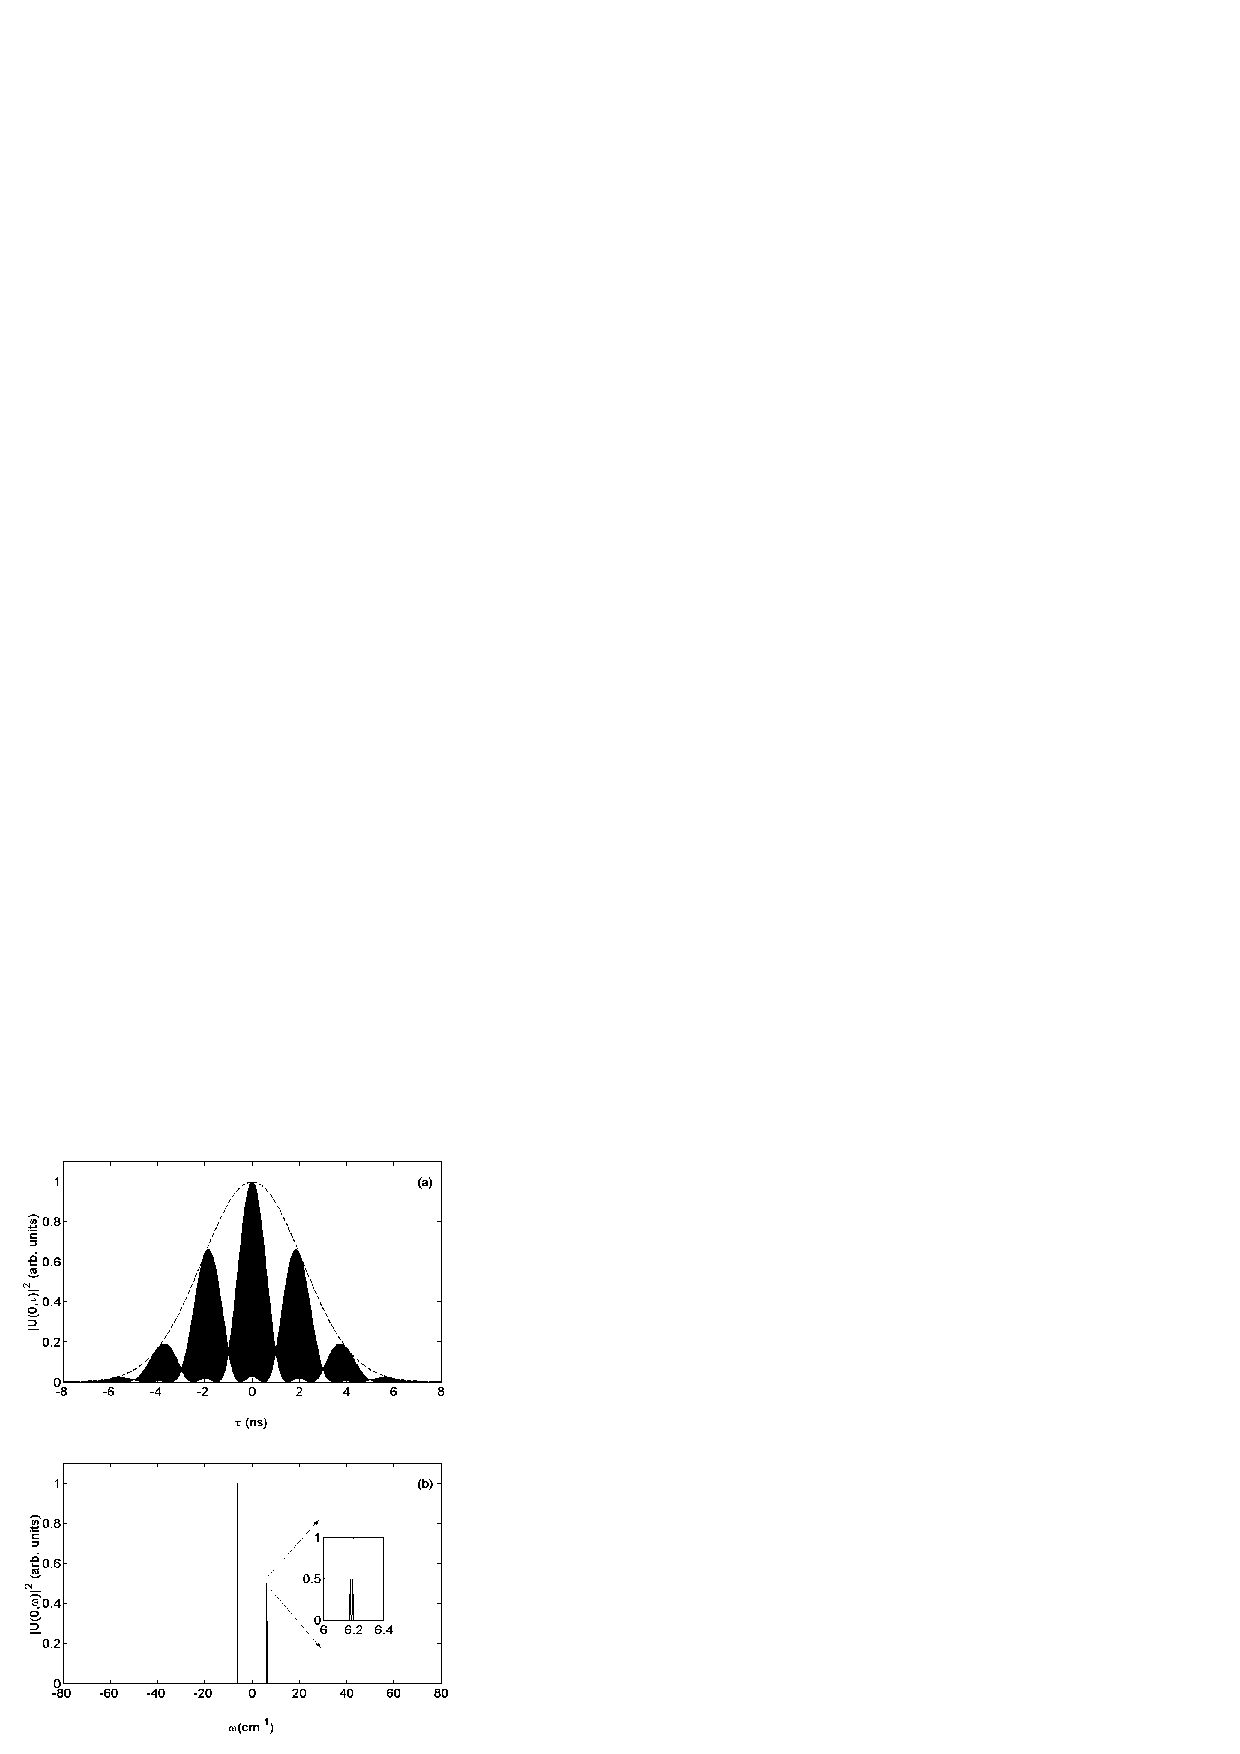
\includegraphics[width=5in]{nlsetime.pdf}
\end{center}
\renewcommand{\baselinestretch}{1}
\small\normalsize
\begin{quote}
\caption[Multimode pulse input toe NLSE]
{Multimode pulse input to the NLSE: (a) input pulse in time
domain and (b) input spectrum.}
\label{figA.1}
\end{quote}
\end{figure}
\renewcommand{\baselinestretch}{2}
\small\normalsize

The basic form of the initial complex wave envelope function is
%A.10
\begin {equation}
U(0,\tau) = exp \left( - {\tau^2 \over 2\tau_p^2} \right)
\left\{
\begin{array}{l}
exp\left( {i\Omega\tau \over 2} \right) + \\
exp\left( - {i\Omega\tau \over 2} \right)
\end{array}
\right\} ,
\end{equation}
where $\tau_p$ is the pulse width T$_p$ =5\,ns FWHM, normalized to the time scale
T$_0$, $\Omega$=366\,GHz is the frequency detuning between the two laser
sources normalized to a frequency scale $\Omega_0$ = 62.5\,MHz.  Figure A.1(a)
shows a plot of this pulse $|U(0,\tau)|^2$. The overall Gaussian envelope
has an FWHM of 5\,ns, the closely spaced dark lines are due to the 366\,GHz
($\sim$3\,ps) beating between the two input pump frequencies. The 2\,ns
modulations on the pulse are due to the 0.5\,GHz mode-structure in the
blue-shifted pump wave. Figure A.1(b) shows the input spectrum of this pulse
which consists of two highly monochromatic pump waves with a detuning of
$\Omega$=366\,GHz. The spectrum of the blue-shifted pump, upon magnification,
is seen to be composed of two very closely spaced peaks, with a separation of
$\Delta\nu$=0.5\,GHz. Hart {\it et al}.\ \cite{hart1} did not use pulsed
wave functions in their NLSE simulations as the size of the FFT required to do
so made it computationally prohibitive at that time. The size of the FFT was
chosen such that it would accommodate a time span of 16\,ns in order to go
sufficiently far into the wings on the Gaussian pulse; and a frequency span of
16\,THz in order to accommodate all the sidebands generated and prevent
spurious effects due to the reflection boundary conditions implicit in the
SSFM algorithm. These considerations dictated the size of the FFT to be
$\geq$(16 THz)$\cdot$(16 ns) = 256000. The nearest power of 2 is
2$^{18} = 262144$, which has been used throughout the present work. The
incorporation of the pulsed nature of the light was found to be necessary in
explaining the dynamics. From the perspective of the coupled amplitude
equations used by Hart {\it et al}.\ \cite{hart1}, the present model is equivalent
to a coupled-ODE model with $2^{18}$ coupled ODEs.

%Figure A.2
\begin{figure}
\begin{center}
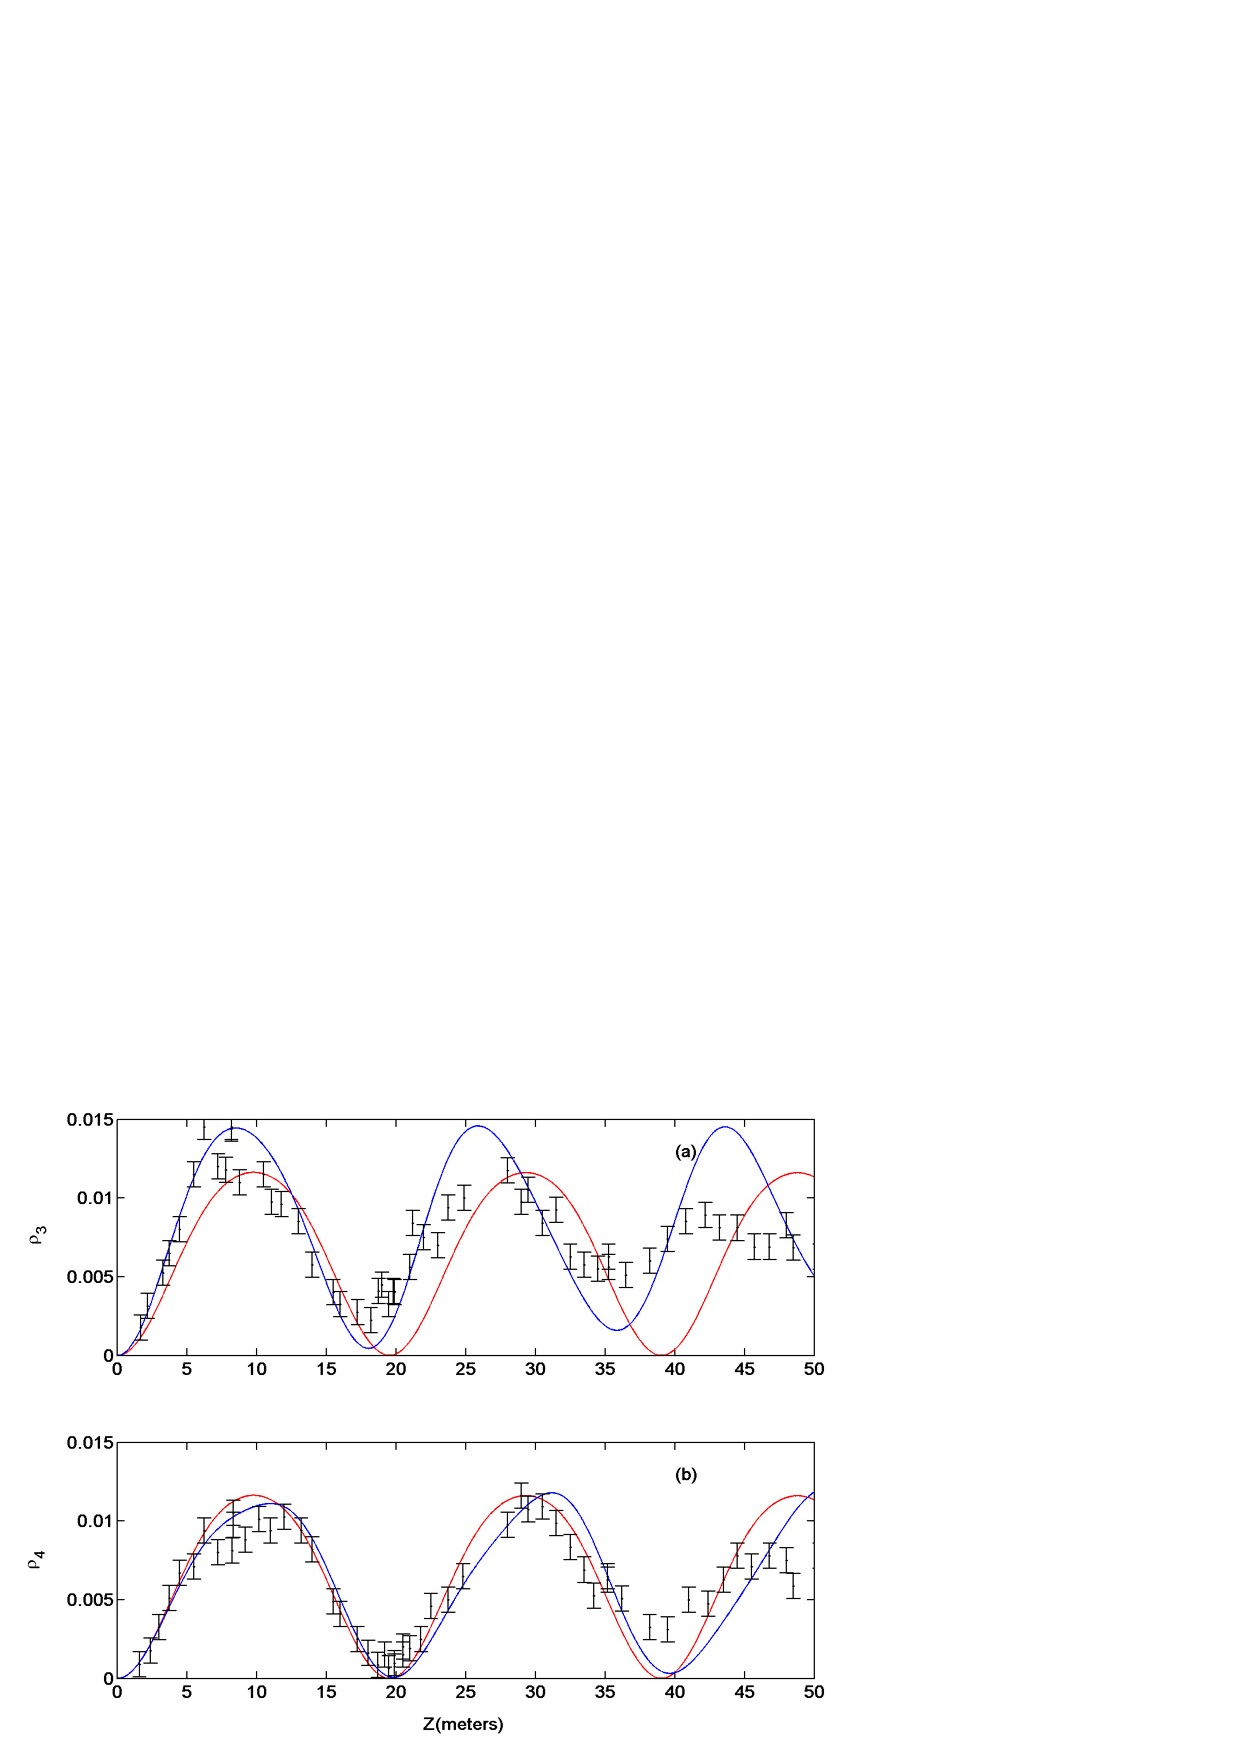
\includegraphics[width=5in]{modestruc21ornot.pdf}
\end{center}
\renewcommand{\baselinestretch}{1}
\small\normalsize
\begin{quote}
\caption[Short caption for Figure A.2.]
{Effects of inclusion of the multimode nature ($\Delta\nu = 0.5$\,GHz) of the blue-shifted input pump laser on the 1st order sideband evolution as a function of fiber length for P$_0 = 2.1$\,W. Dashed curves represent simulations without the multimode nature and solid curves represent simulations with the multimode nature. $\Omega = 366$\,GHz, $\gamma = 0.019$\,W$^{-1}$\,m$^{-1}$, and $\beta^{(2)} = 55$\,ps$^2$/km (a) power in the blue-shifted sideband, (b) power in the red-shifted sideband.}
\label{figA.2}
\end{quote}
\end{figure}
\renewcommand{\baselinestretch}{2}
\small\normalsize

%Figure A.3
\begin{figure}
\begin{center}
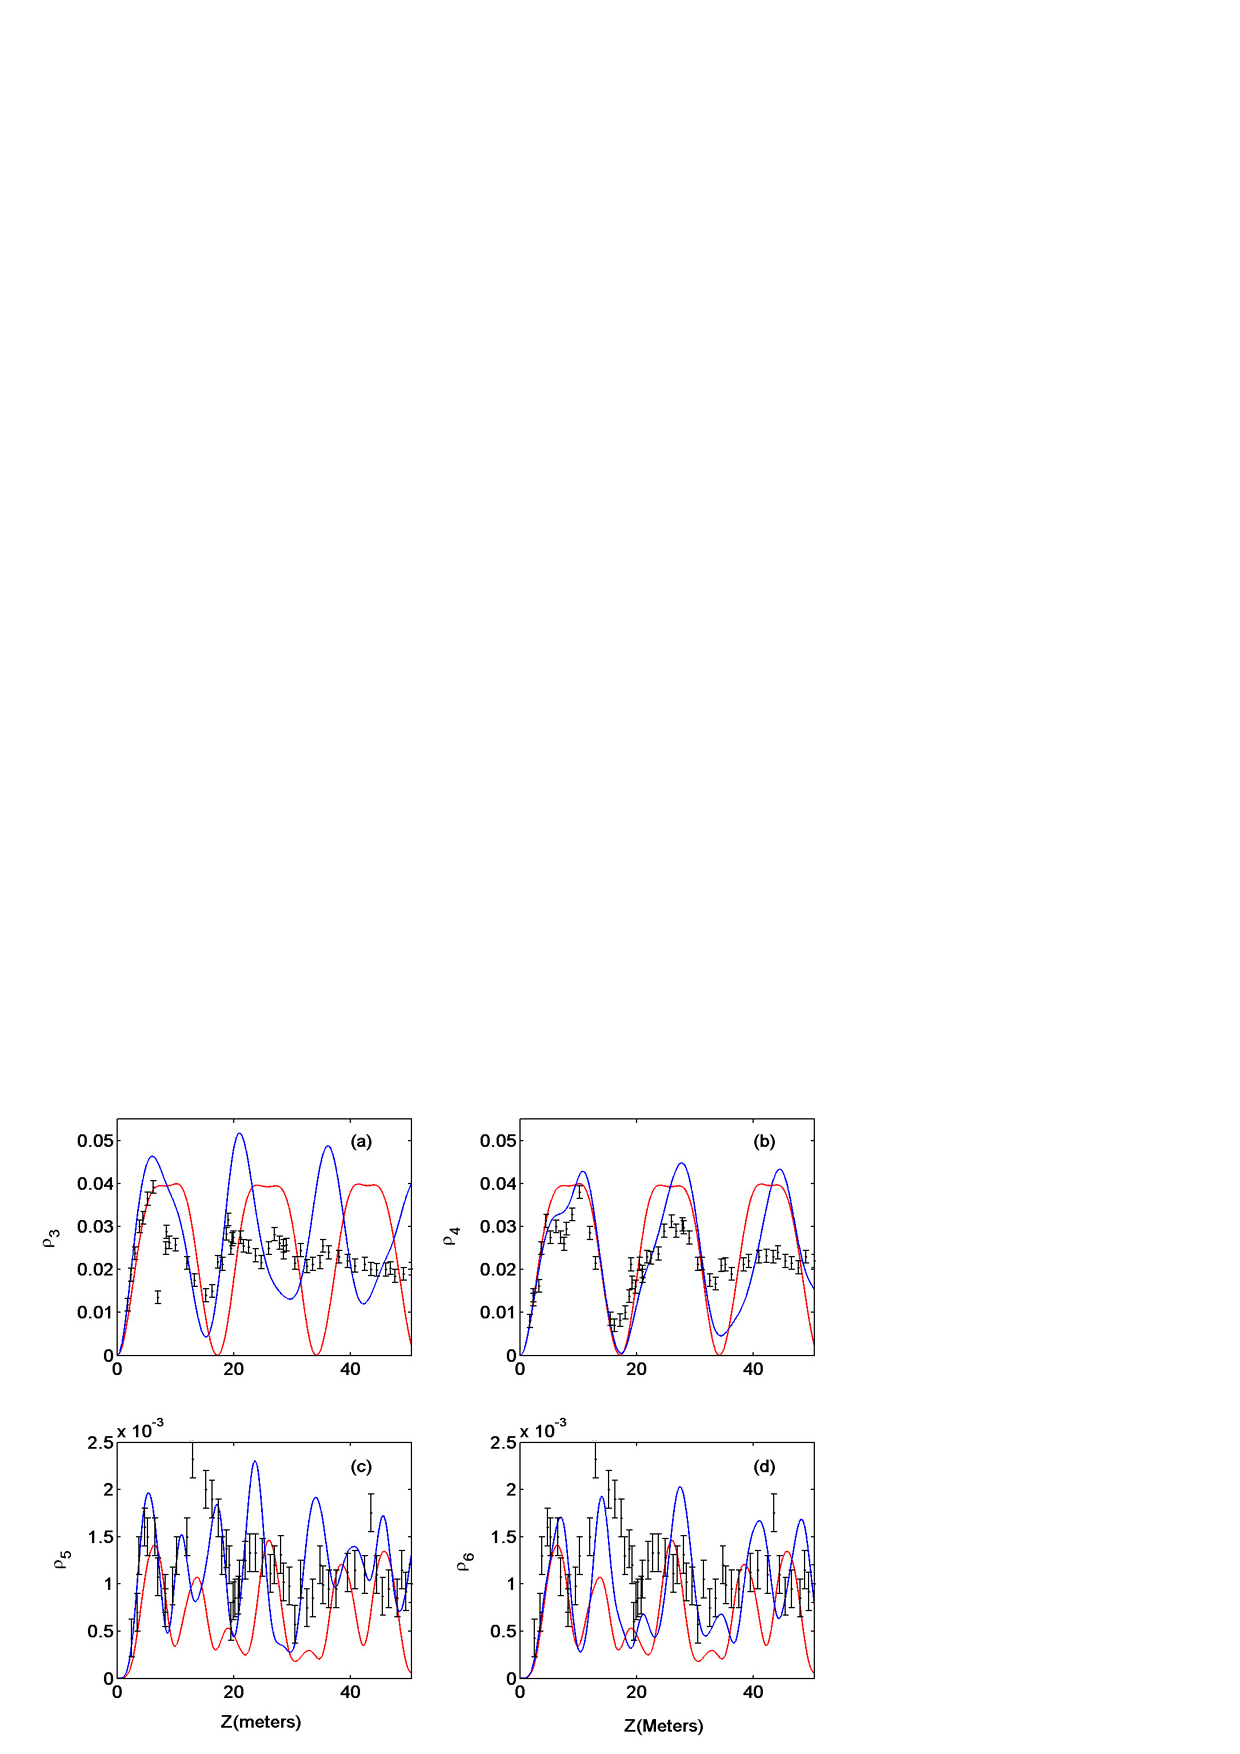
\includegraphics[width=5in]{modestruc55ornot.pdf}
\end{center}
\renewcommand{\baselinestretch}{1}
\small\normalsize
\begin{quote}
\caption[Effects of inclusion of the multimode nature]
{Effects of inclusion of the multimode nature ($\Delta\nu = 0.5$\,GHz) of the blue-shifted input pump laser on the 1st order sideband evolution as a function of fiber length for P$_0 = 5.5$\,W. Dashed curves represent simulations without the multimode nature and solid curves represent simulations with the multimode nature. $\Omega = 366$\,GHz, $\gamma = 0.019$\,W$^{-1}$\,m$^{-1}$, and $\beta^{(2)} = 55$\,ps$^2$/km (a) power in the first-order blue-shifted sideband, (b) power in the first-order red-shifted sideband, (c) power in the second-order blue-shifted sideband, (d) power in the second-order red-shifted sideband.}
\label{figA.3}
\end{quote}
\end{figure}
\renewcommand{\baselinestretch}{2}
\small\normalsize

%Figure A.4
\begin{figure}
\begin{center}
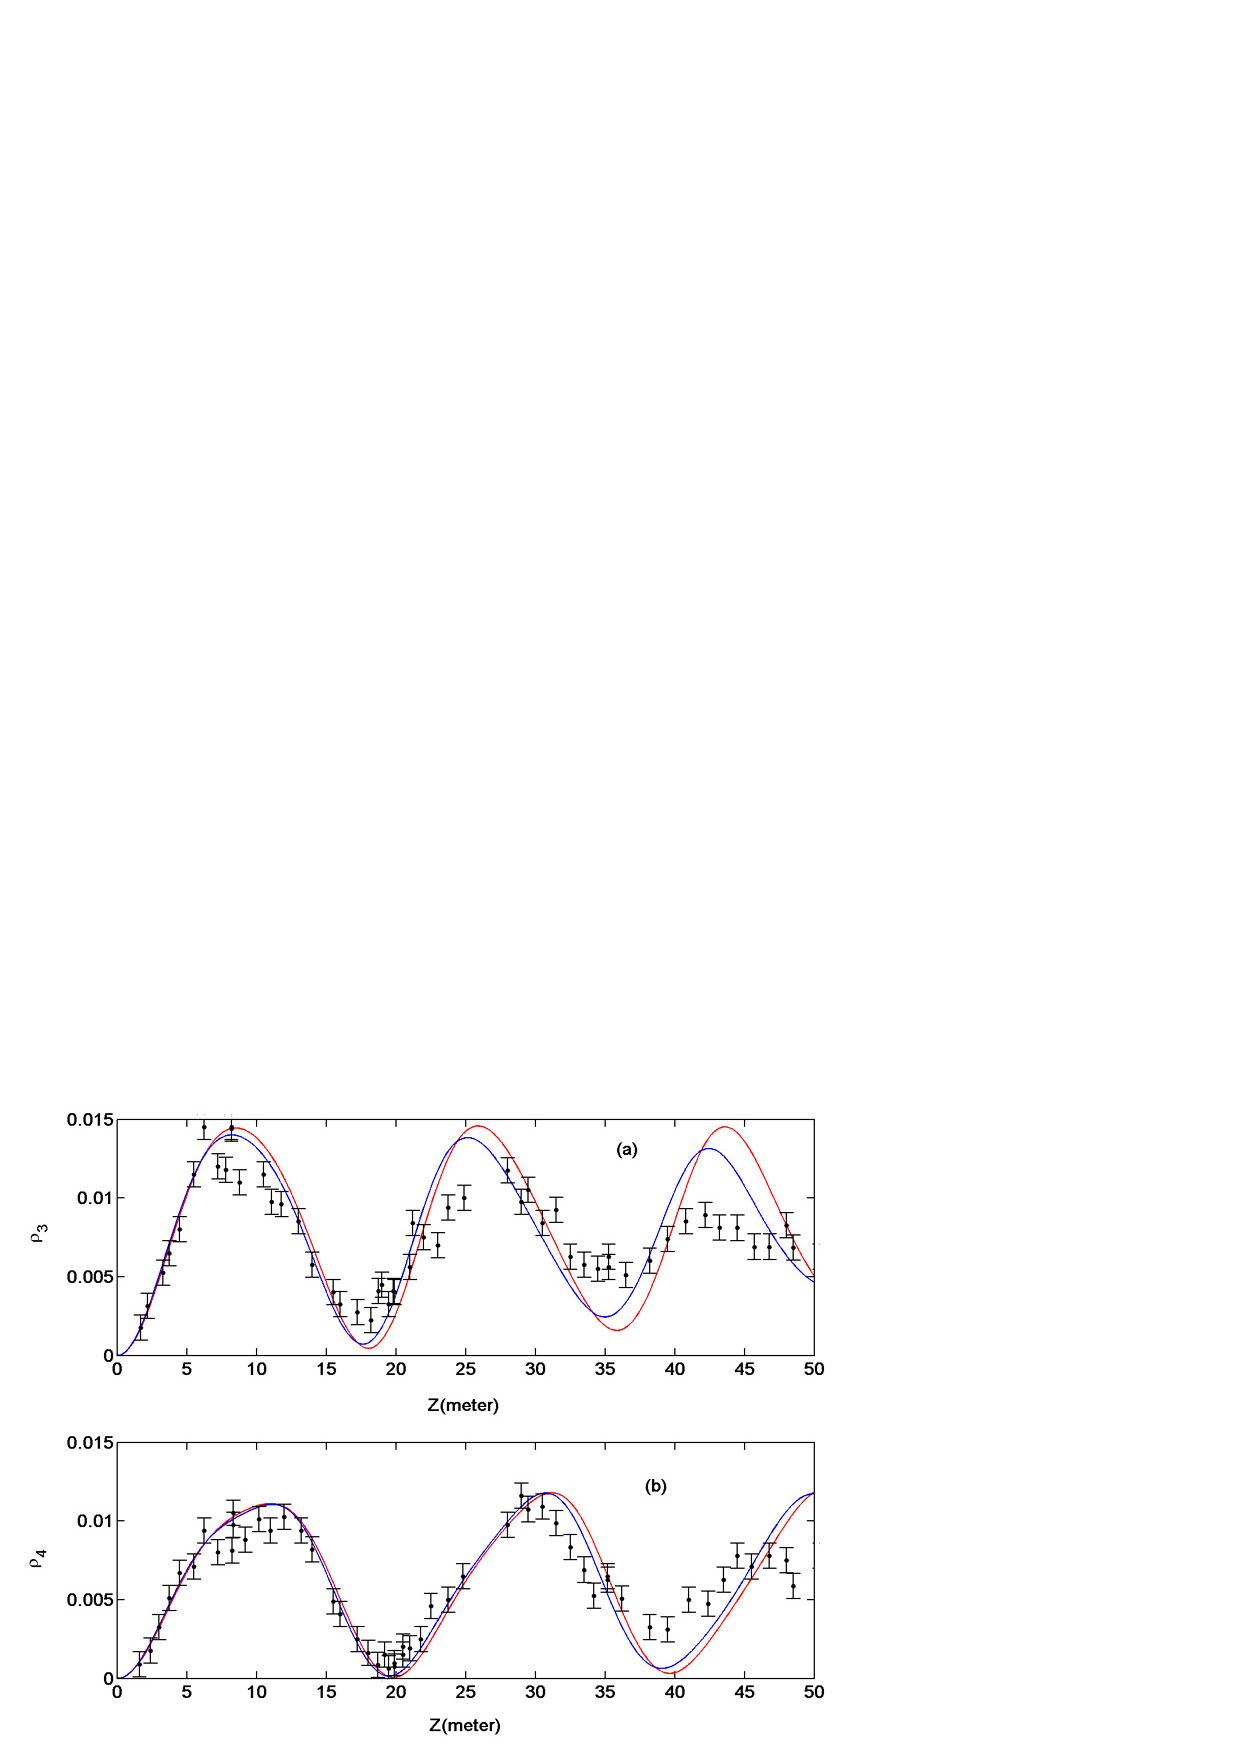
\includegraphics[width=5in]{nlsez21cwpulse.pdf}
\end{center}
\renewcommand{\baselinestretch}{1}
\small\normalsize
\begin{quote}
\caption[Effects of inclusion of the pulsed nature]
{Effects of inclusion of the pulsed nature (5\,ns FWHM) of the input pump laser light on the first-order sideband evolution as a function of fiber length for P$_0 = 2.1$\,W. Dashed curves represent cw simulations and solid curves represent pulsed simulations. $\Omega = 366$\,GHz, $\Delta\nu = 0.5$, $\gamma = 0.019$\,W$^{-1}$m$^{-1}$, and $\beta^{(2)} = 55$\,ps$^2$/,km (a) power in the blue-shifted sideband, (b) power in the red-shifted sideband.}
\label{figA.4}
\end{quote}
\end{figure}
\renewcommand{\baselinestretch}{1}
\small\normalsize

%Figure A.5
\begin{figure}
\begin{center}
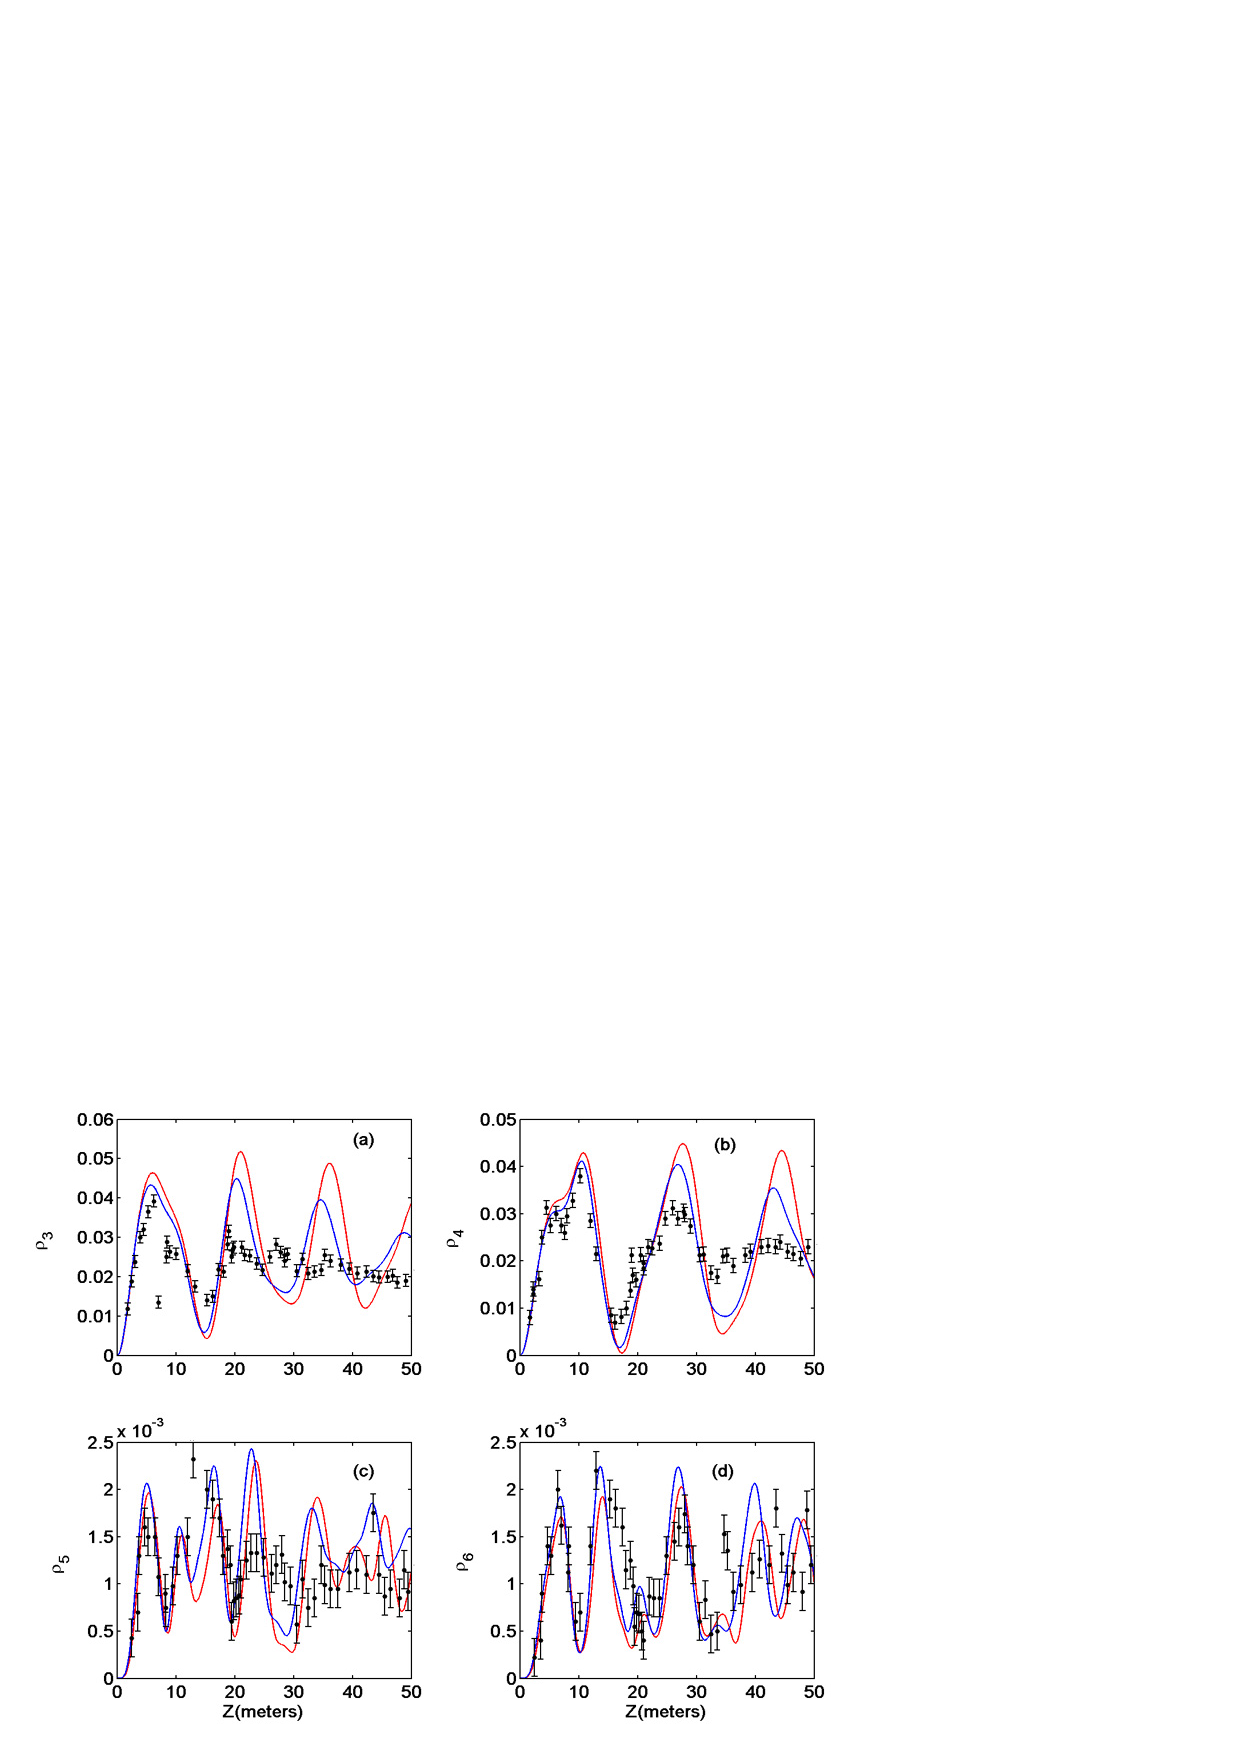
\includegraphics[width=5in]{nlsez55cwpulse.pdf}
\end{center}
\renewcommand{\baselinestretch}{1}
\small\normalsize
\begin{quote}
\caption
[Other effects of inclusion of the pulsed nature]
{Effects of inclusion of the pulsed nature (5\,ns FWHM) of the input pump laser on the first- and second-order sideband evolution as a function of fiber length for P$_0 = 5.5$\,W. Dashed curves represent cw simulations and solid curves represent pulsed simulations. $\Omega = 366$\,GHz, $\Delta\nu = 0.5$, $\gamma = 0.019$\,W$^{-1}$m$^{-1}$, and $\beta^{(2)} = 55$\,ps$^2$/,km (a) power in the first-order blue-shifted sideband, (b) power in the first-order red-shifted sideband, (c) power in the second-order blue-shifted sideband, (d) power in the second-order red-shifted sideband.}
\label{figA.5}
\end{quote}
\end{figure}
\renewcommand{\baselinestretch}{2}
\small\normalsize

Upon incorporation of the multimode nature of the blue input pump laser source
and the stochastic fluctuations in the initial power in the lasers, the
initial wave function takes the form
%A.11
\begin{equation}
U(0,\tau) = exp\left( - {\tau^2 \over 2\tau_p^2} \right)
\left\{
\begin{array}{l}
\sqrt{{1 + \delta\rho_1 \over 2}}
\left[ \begin{array}{l}
exp \left( {i(\Omega+\Delta\nu)\tau \over 2} \right) + \\
exp \left( {i(\Omega-\Delta\nu)\tau \over 2} \right)
\end{array} \right]\\
+ \sqrt{1 + \delta\rho_2} exp\left( - {i\Omega\tau \over 2} \right)
\end{array}
\right\}.
\end{equation}

\

\noindent $\Delta\nu = 0.5$\,GHz is the frequency separation between the two longitudinal
modes in the blue-shifted pump. $\delta\rho_1$ and $\delta\rho_2$ are
Gaussian random deviates (generated using the Box-Muller algorithm
\cite{boxmuller}) that represent the initial power fluctuations in each of the
pump laser sources. Their standard deviations were taken to be,
$\sigma_{\rho_1} = 0.2$, $\sigma_{\rho_2} = 0.11$ for simulations from 0\,m to
20\,m, $\sigma_{\rho_1} = 0.12$, $\sigma_{\rho_2} = 0.05$ for simulations from
20\,m to 50\,m along the length of the fiber. This is exactly the same
prescription used by Hart {\it et al}.\ \cite{hart1} in their simulations and is
dictated by their experimental measurements of the fluctuations in the pump
laser intensities.

At this point it is worth noting the effects of the inclusion of two attributes of
the input laser light, namely, the multimode nature of the blue-shifted pump, and
the pulsed nature of the input light (assumed to be cw in the simulations reported by
Hart {\it et al}.\ \cite{hart1}).

Figure A.2 shows a comparison between simulations with (solid curves) and without (dashed curves) the multimode nature for an input pump power of 2.1 Watts. The simulations with the mode structure show the asymmetry between the blue- and red-shifted sideband evolution, in particular, the difference in spatial wavelength between the two, and a non-return to zero nature of the evolution, as observed in the experimental data (black dots with error bars). These features are absent in the simulations without mode-structure. $\rho_3$ and $\rho_4$ stands for the first order blue- and red-shifted sidebands respectively.  Figure 2.3 shows the corresponding comparison for the case of 5.5 Watts of input pump power.  Here, too, the simulations incorporating the multimode nature of the blue-shifted pump (solid curves) are seen to be an improvement over those not incorporating it (dashed curves). A feature of the experimental data (black dots with errorbars) is that for the $\rho_3$ sideband, the initial part of the evolution involves a peak followed by a shoulder, while for the $\rho_4$ sideband, the initial part of the evolution involves a shoulder followed by a peak. This feature, too, is seen to occur as a result of the inclusion of the multimode nature of the blue-shifted pump.

The effect of inclusion of the pulsed nature of the input beam is seen in Fig.\ A.4 (for the 2.1 Watt case) and Fig.\ A.5 (for the 5.5 Watt case). The solid dashes represent simulations for a cw input beam and the solid curves represent those for a pulsed input beam. The incorporation of the pulsed nature clearly results in damping of the sideband trajectories which are seen to come closer to the experimental data \cite{hart1} (black dots with error bars).

Use of the FFT algorithm makes evaluation relatively fast compared to other
finite-difference schemes. The computational error is $O(\Delta z^2)$, thus
the solution converges with decreasing spatial step-size $\Delta z$.

The simulations were tested for the conservation of total power along the
fiber length (by setting the loss $\alpha$ to zero) and for the conservation
of asymmetry \cite{thompson1,hart1} given by
%A.12
\begin{equation}
C(Z) = \sum_{i=1}^{\infty}(2i-1)[\rho_{2i-1}(Z)-\rho_{2i}(Z)] .
\end{equation}

A clearer picture of the evolution of the sidebands is obtained by plotting both the
power in the sidebands and their standard deviations as a function of length along the fiber. Figures A.6(a) and A.6(b) show a comparison between simulation and experiment of the evolution
of the first-order blue-shifted ($\rho_3$) and red-shifted ($\rho_4$) sidebands,
respectively, for an input power of 2.1 W. The dashed curves represent NLSE simulations
which include the stochastic nature of the input powers of the pump lasers but exclude
the stochastic phase fluctuations added along the length of the fiber, an attribute
which is included in the simulations represented by the solid curves. The black dots
with error bars represent the experimental data. The measured sideband
power, normalized to the total power in the fiber, is periodic in length but
appears to be damping to a constant value. The measured data also show a clear
difference between the spatial wavelengths of oscillation of the blue-shifted ($\rho_3$) and red-shifted ($\rho_4$) sidebands trajectories, respectively. Both these features are captured well by both the simulations. Figures A.6(c) and A.6(d) compare experimental and simulated
measures of the evolution of the standard deviation in the sideband power
along the fiber length. It is clearly observed that simulations with phase noise
added to the light field along the length of the fiber (solid curves) are closer to the
experimental data as compared to those that exclude this feature (dashed curves). This indicates
the instrumental nature of the phase fluctuations in explaining key features of the dynamics.

%Figure A.6
\begin{figure}
\begin{center}
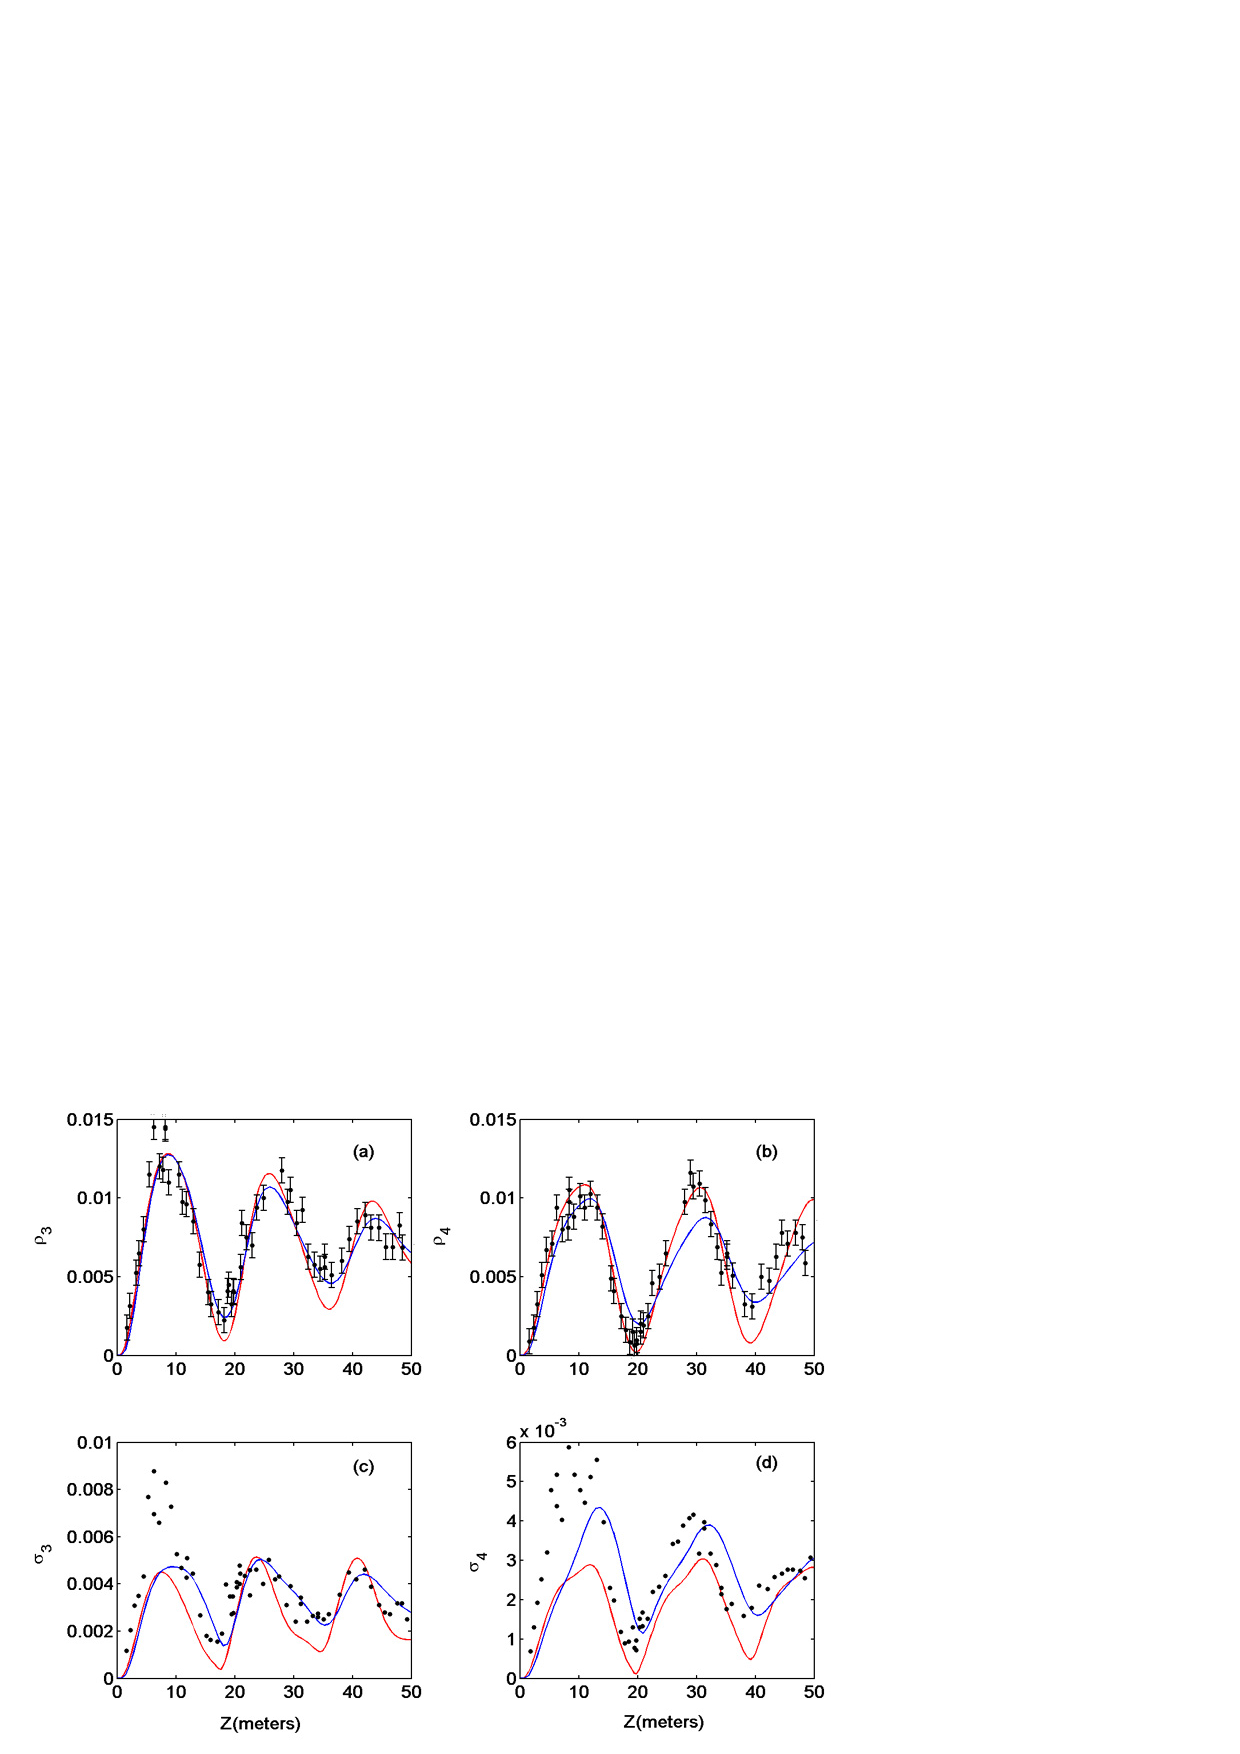
\includegraphics[width=5in]{nlsez21phaseornot.pdf}
\end{center}
\renewcommand{\baselinestretch}{1}
\small\normalsize
\begin{quote}
\caption
[Comparison between experiments measurements]
{Comparison between the experimental measurements \cite{hart1}(black), the random initial condition NLSE model excluding phase noise (dashed curves) and the stochastic phase noise NLSE model (solid curves) showing the first-order sideband evolution as a function of fiber length for P$_{0} = 2.1$\,W, $\Omega = 366$\,GHz, $\Delta\nu = 0.5$\,GHz,$\gamma = 0.019$\,W$^{-1}$m$^{-1}$, and $\beta^{(2)} = 55$ps$^2$/km: dynamical evolution of the: (a) power in the blue-shifted sideband, (b) power in the red-shifted sideband, (c) fluctuations in the blue-shifted sideband, (d) fluctuations in the red-shifted sideband.}
\label{figA.6}
\end{quote}
\end{figure}
\renewcommand{\baselinestretch}{2}
\small\normalsize

The apparent damping of the periodic sideband trajectory is seen more
dramatically in Figs.\ A.7(a) and A.7(b), which show the evolution of the
first-order sideband power along the fiber for an input power of 5.5\,W.
The two first-order sidebands evolve differently. They appear to
damp to a constant value at a faster rate than for the case with an input pump
power of 2.1\,W. Here again, NLSE simulations that incorporate phase noise along the length
of the fiber (solid curves) are much more successful in accurately capturing the dynamical features of the system than NLSE simulations that do not take this feature into account (dashed curves).  Figures A.7(c) and A.7(d) show a comparison between the simulated and measured standard deviations. Comparisons for the second-order blue-shifted ($\rho_5$) and red-shifted ($\rho_6$) sidebands, respectively, are shown in Figs.\ A.7(e) and A.7(f).


%Figure A.7
\begin{figure}
\begin{center}
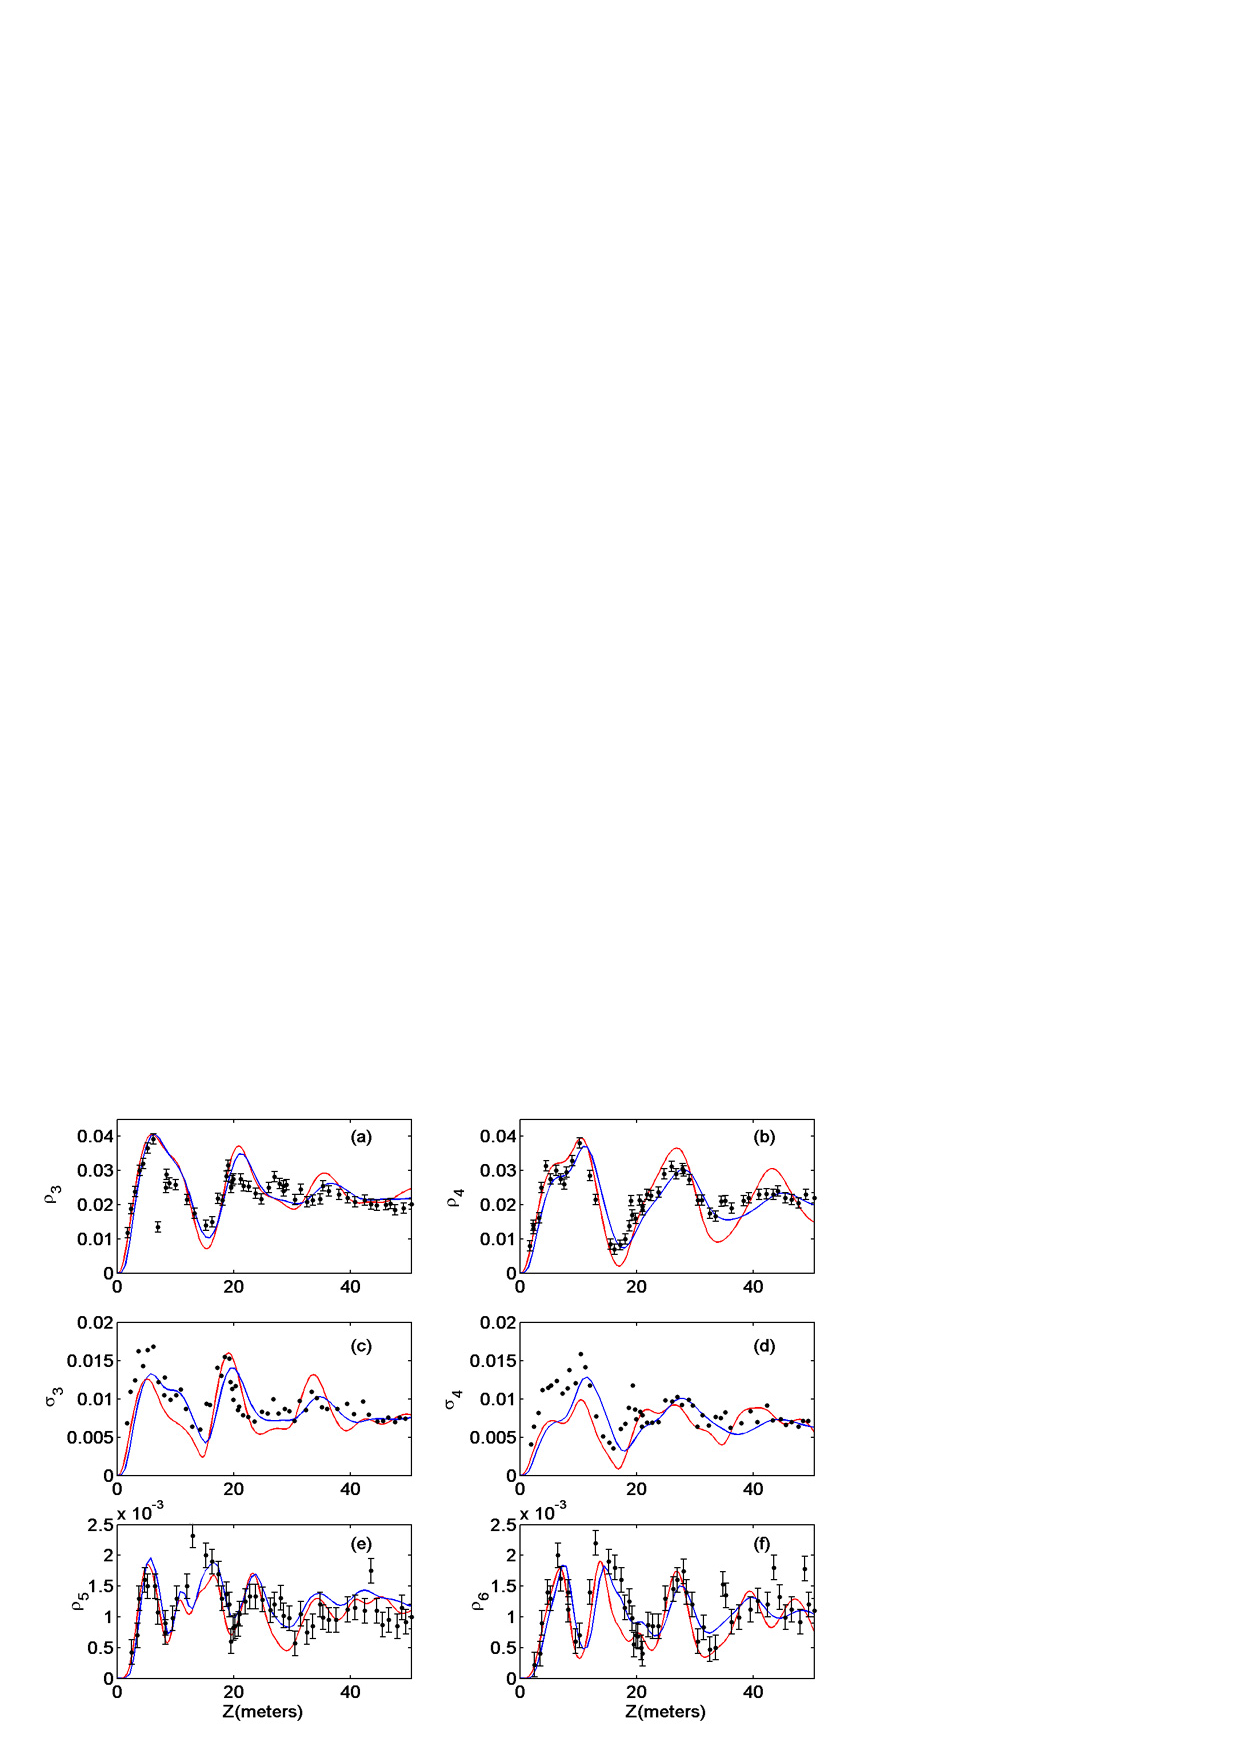
\includegraphics[width=5in]{nlsez55phaseornot.pdf}
\end{center}
\renewcommand{\baselinestretch}{1}
\small\normalsize
\begin{quote}
\caption
[This figure caption is indented and single-spaced]
{This figure caption is indented and single-spaced.  Comparison between the experimental measurements \cite{hart1} (black), the random initial condition NLSE model excluding phase noise (dashed curves) and the stochastic phase noise NLSE model (solid curves) showing the first- and second-order sideband evolution as a function of fiber length for P$_{0} = 5.5$\,W, $\Omega = 366$\,GHz, $\Delta\nu = 0.5$\,GHz, $\gamma = 0.019$\,W$^{-1}$m$^{-1}$, and $\beta^{(2)} = 55$\,ps$^2$/km: dynamical evolution of the: (a) power in the first-order blue-shifted sideband, (b) power in the first-order red-shifted sideband, (c) fluctuations in the first-order blue-shifted sideband, (d) fluctuations in the first-order red-shifted sideband, (e) power in the second-order blue-shifted sideband, (f) power in the second-order red-shifted sideband.}
\label{figA.7}
\end{quote}
\end{figure}
\renewcommand{\baselinestretch}{2}
\small\normalsize

The observed dynamical evolution of the sidebands is found to depend
sensitively on the strength of the stochastic phase fluctuations. Yet, best
agreement with the experimental results of Hart {\it et al}.\ \cite{hart1} is
achieved with exactly the same noise strength $\sigma^2_\phi$ as used in
their truncated ODE model, namely, $\sigma^2_\phi = 0.0067$\,m$^{-1}$. They
report that including phase noise in their FWM calculations resulted in a
spurious linear drift in the trajectories for the sideband power with length.
To remove this artifact of the computations, they added a linear loss to their
coupled ODEs. They set the loss coefficient $\alpha = 0.0046$\,m$^{-1}$ by
finding the value that removed this increasing slope. We have observed exactly
the same secular growth phenomenon for a wide range of the noise strength
$\sigma^2_\phi$ and have arrived at an empirical prescription for $\alpha$
namely, $\alpha\sim\sigma^2_\phi$, where $\sigma^2_\phi$ is the
variance of the added phase noise. This indicates the general nature of
dynamics resulting from the addition of stochastic, $\delta$-correlated phase
fluctuations to systems governed by nonlinear partial differential equations
\cite{risken}.

It is remarkable that the strength of the phase noise required is the same in
both the 2.1\,W and the 5.5\,W cases. Further, it is worth noting that exactly
the same noise strength was used by Hart {\it et al}.\ \cite{hart1}, the difference
being that they introduced phase noise only in the pump frequencies, whereas
we have introduced it in all the Fourier modes ($\sim2^{18}$). As a
confirmation of this result, they also performed experiments and numerical
simulations examining the sideband power dependence on the input power at a
fixed length of 50.4\,m of the same fiber. We have repeated these simulations
with the stochastic NLSE model and the results are shown in Figs.\ 2.8(a)
(blue-shifted sideband) and 2.8(b) (red-shifted sideband). The experimental
measurements of the sideband powers are represented by filled squares and the
results of numerical simulations are represented by triangles (without phase
noise) and by circles (with phase noise). The simulations are seen to follow
the general trend seen in the experiments. As the pump power is increased, the
triangles (without phase noise) start to disagree with experiment, whereas the
circles (with phase noise) are much closer to experiment. The phase noise
strength used in these simulations was exactly the same as that used in the
simulations depicted in Figs.\ A.6 and A.7. The agreement between the phase noise
simulations and the experimental data was (once again) highly sensitive to the
noise strength. Since this experiment (unlike those shown in Figs.\ A.2 - A.7)
is non-destructive, it can be used to deduce the strength of phase noise
processes in a given optical fiber. It will be shown in Sec.\ 2.4 that a
likely cause of the phase noise is fluctuation in the linear refractive index
of the fiber. The noise strength deduced from the present computational study
corresponds to a refractive index inhomogeneity of
$\langle \Delta n^{2} \rangle \sim 10^{-16}$.

%Figure A.8
\begin{figure}
\hspace{1.25in}
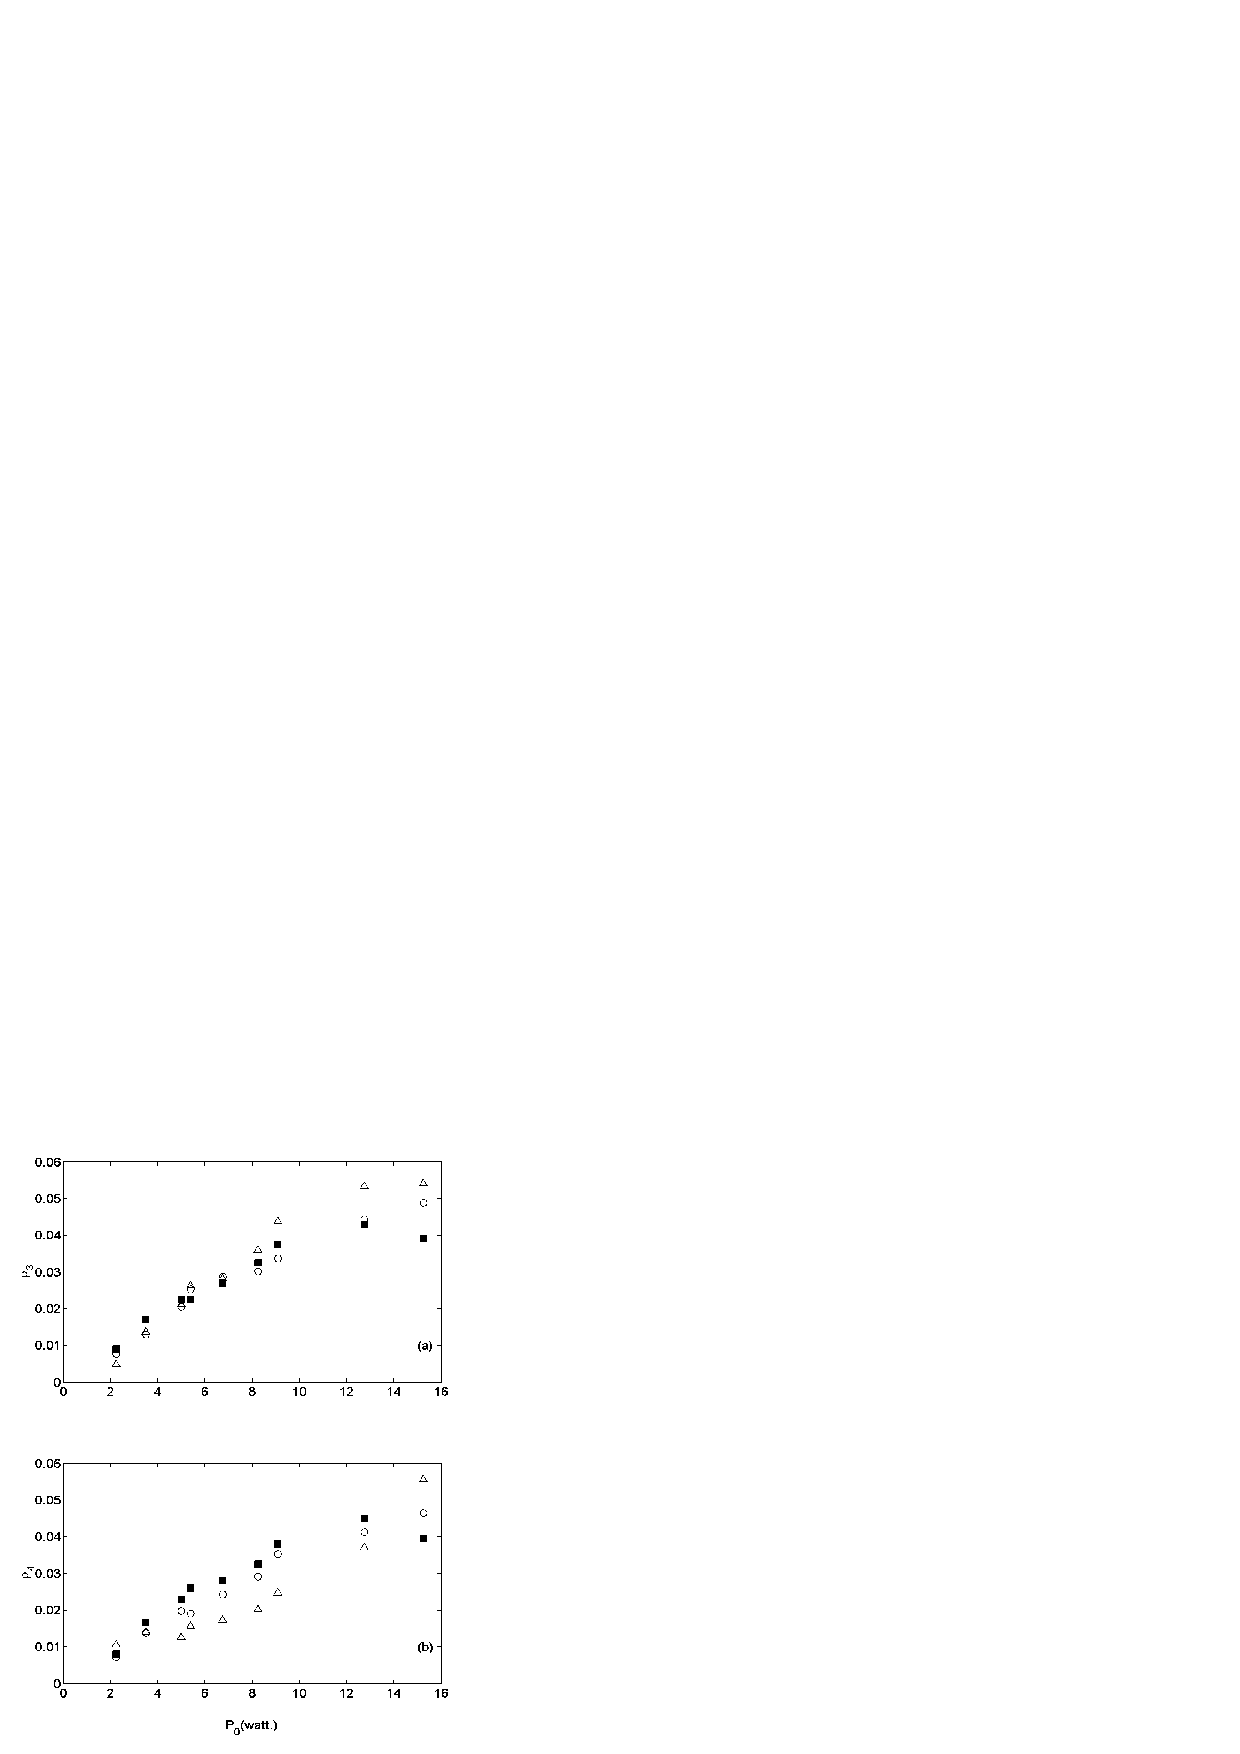
\includegraphics[width=5in]{nlsefinal.pdf}
\renewcommand{\baselinestretch}{1}
\small\normalsize
\begin{quote}
\caption
[Comparison between the experiments measurements (filled squares)]
{Comparison between the experimental measurements (filled squares), simulations without stochastic phase fluctuations (open triangles) and with stochastic phase fluctuations (open circles) of the first-order sideband power versus pump input power for L=50.39\,m, and $\Omega = 366$\,GHz: power in the (a) blue-shifted sideband and (b) red-shifted sideband.}
\label{figA.8}
\end{quote}
\end{figure}
\renewcommand{\baselinestretch}{2}
\small\normalsize

%Figure A.9
\begin{figure}
\begin{center}
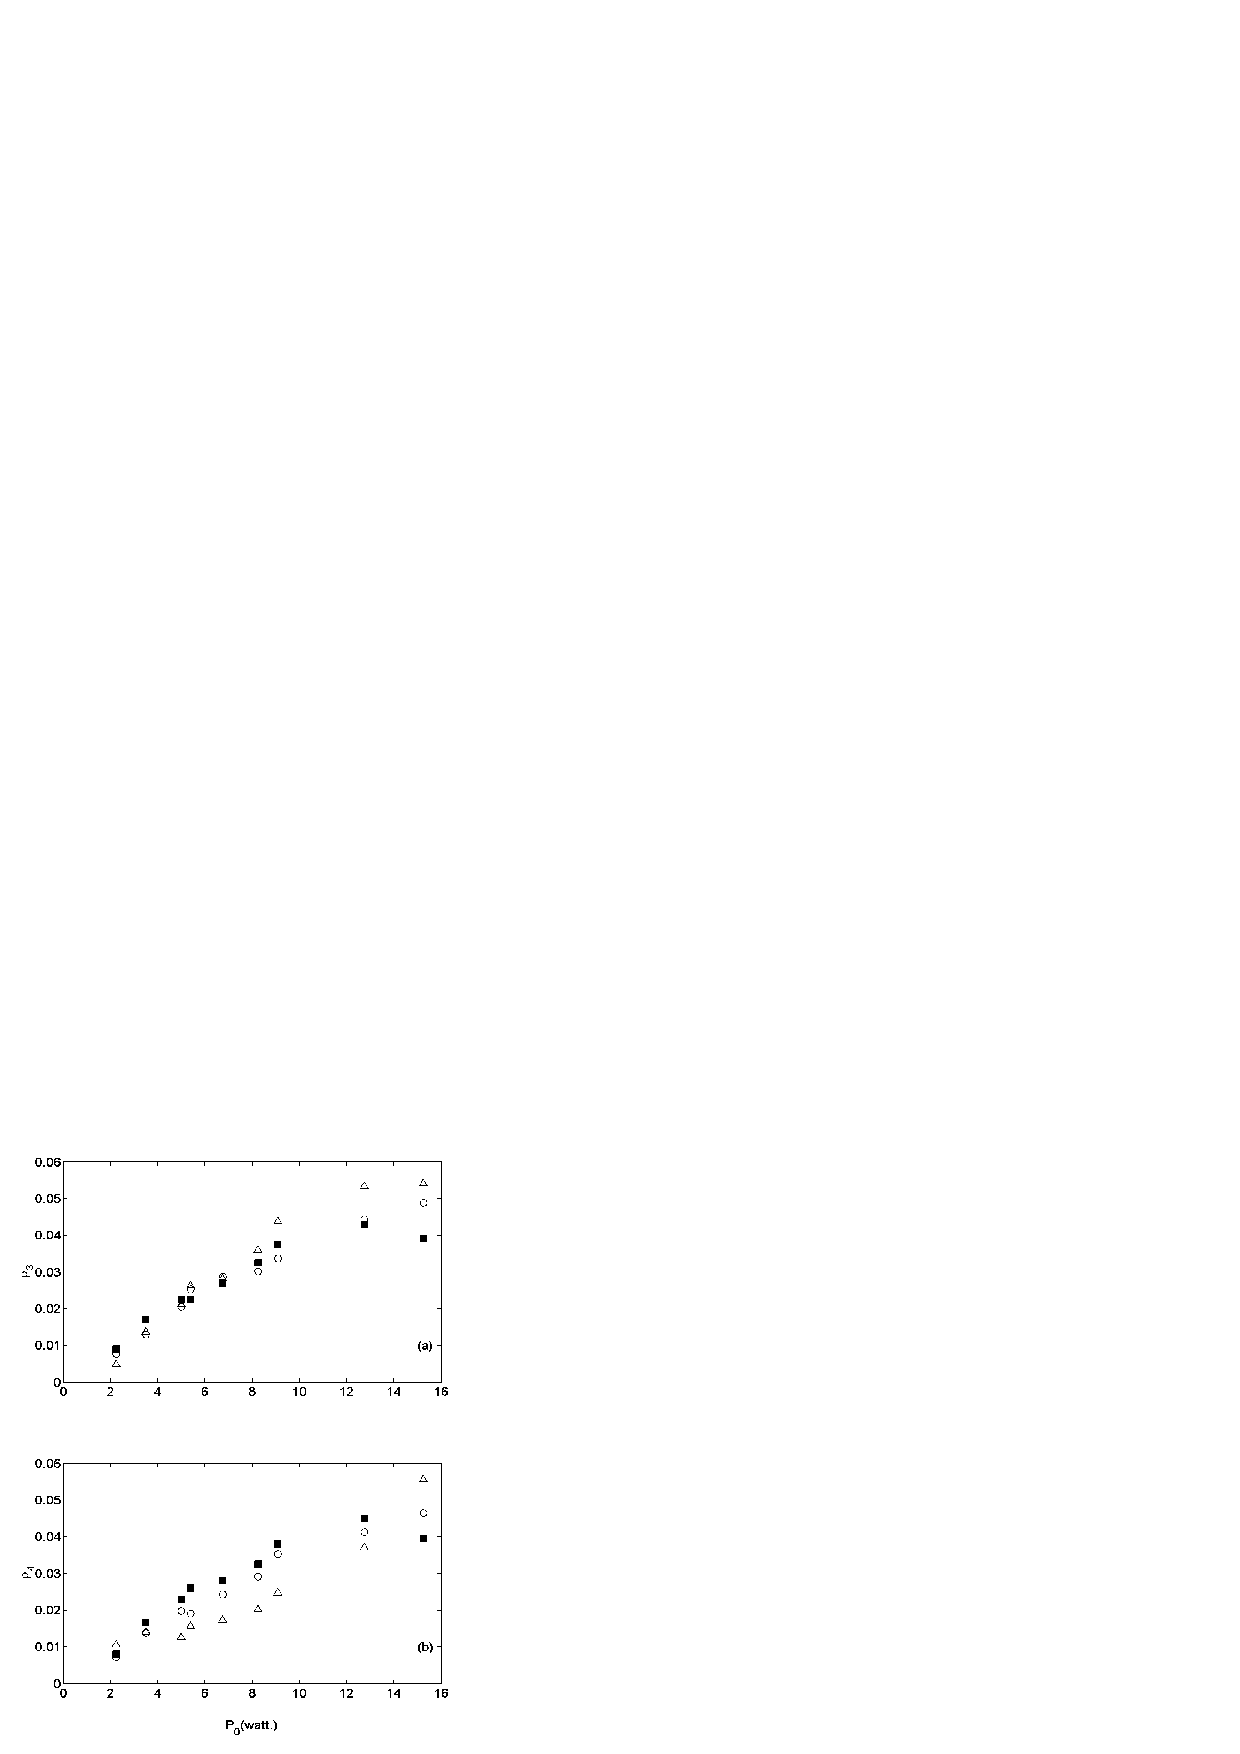
\includegraphics[width=5in]{nlsefinal.pdf}
\end{center}
\renewcommand{\baselinestretch}{1}
\small\normalsize
\begin{quote}
\caption
[Evolution of the FWM spectrum]
{Evolution of the FWM spectrum along the fiber (a) P=2.1\,W, experiment, (b) P=5.5\,W, experiment, (c) P=2.1\,W, stochastic-NLSE model, (d) P=5.5\,W, stochastic-NLSE model.}
\label{figA.9}
\end{quote}
\end{figure}
\renewcommand{\baselinestretch}{2}
\small\normalsize

Till now the comparisons between our simulations of the full NLSE and the
truncated ODE model give basically the same results, although with much better
agreement with experiment. However, the full NLSE can also provide a detailed
comparison with the experimental spectra. This was not available from the
truncated ODE model. The simulations reported in this work were carried out
with a very high frequency and time resolution in order to incorporate the
fact that the input light was not cw, but was composed of $\sim$ 5\,ns long
pulses; and that the number of sidebands generated required the frequency
spread of the FFT to be $\sim$ 16\,THz, while resolving a longitudinal
mode-structure of $\Delta\nu$ $\sim 0.5$\,GHz. The spectral resolution used was
$\sim$ 0.05\,GHz, whereas the spectrometer used to observe the spectra had a
resolution 1000 times larger ($\sim$ 50\,GHz). To account for this difference,
the simulated spectra were first convolved with a Gaussian of unit peak and
62\,GHz FWHM, before they were compared with the observed spectra.

Figures A.9(a) and A.9(b) show three-dimensional plots of the average experimental
FWM output spectrum along the length of the fiber for input pump powers of 2.1\,W and 5.5\,W,
 respectively (courtesy Hart {\it et al}.\ \cite{hart1}). The vertical
axis represents the intensity, normalized to the peak power in one of the
input pumps, plotted on a logarithmic scale. The pump frequencies are centered
on $+/-\Omega/2$ and the fiber length is increasing into the page. Figures
9(c) and 9(d) show the corresponding comparisons based on simulations using
the stochastic-NLSE model. The basic features of the spectral evolution are
captured by the simulations.

%Figure  A.10
\begin{figure}
\begin{center}
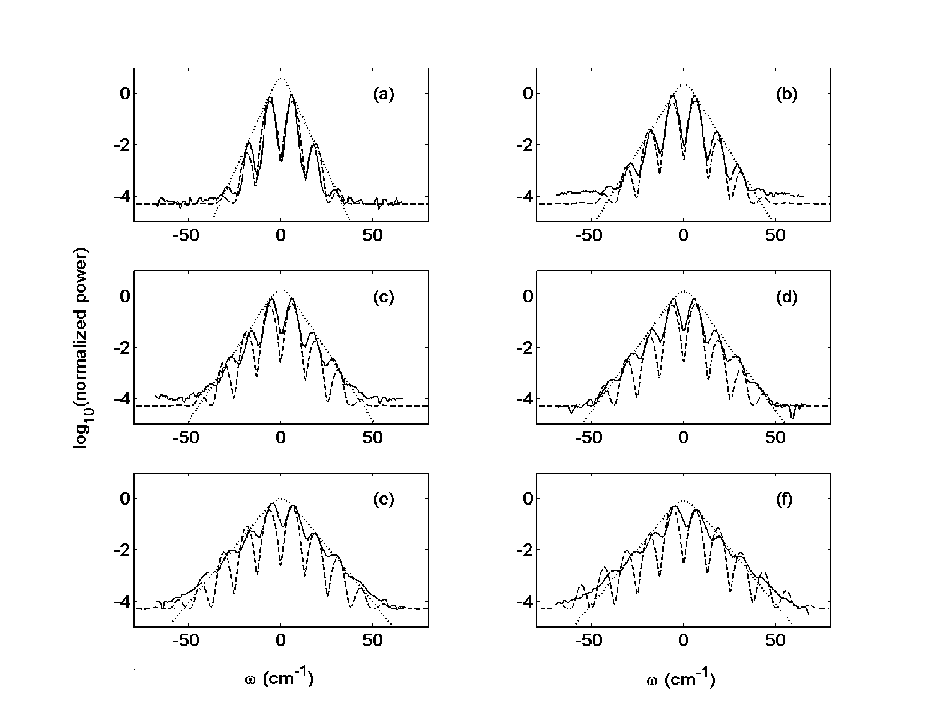
\includegraphics[width=5in]{nlsespec.eps}
\end{center}
\renewcommand{\baselinestretch}{1}
\small\normalsize
\begin{quote}
\caption
[Experimental FWM output spectrum]
{Experimental FWM output spectrum (solid line), convolved spectra from simulations of the stochastic NLSE model (dashed line), and hyperbolic secant envelope fit (dotted line) for pump input powers P$_0$ of (a) 2.1\,W, (b) 5.5\,W, (c) 6.7\,W, (d) 8.3\,W, (e) 12.7\,W, (f) 17.4\,W, fiber length L$= 50.39$\,m, $\Omega = 366$\,GHz, $\Delta\nu = 0.5$\,GHz, $\gamma = 0.019$\,W$^{-1}$m$^{-1}$, and $\beta^{(2)} = 55$\,ps$^2$/km.}
\label{figA.10}
\end{quote}
\end{figure}
\renewcommand{\baselinestretch}{2}
\small\normalsize

Hart {\it et al}.\ \cite{hart1} also documented the experimentally observed FWM
output spectra for a fixed fiber length of 50.39 meters for 6 different input
pump powers. They state the coefficients A and B of the hyperbolic secant
envelopes that best fit the output spectra which are given by
%A.13
\begin{equation}
f(\omega) = Asech(B\omega) ,
\end{equation}
where A and B are the experimental fit parameters.

The hyperbolic secant parameters A and B, that best fit the simulated spectra
are exactly the same as those that best fit the experimental spectra
\cite{hart1} for all the 6 cases of input power considered. Figure 2.10 shows an
overlap of the simulated spectra (dashed line), with the experimental spectra
(solid line) and the experimental hyperbolic secant envelope (dotted line) for
6 different pump powers, namely, (a) 2.1\,W, (b) 5.5\,W, (c) 6.7\,W, (d) 8.3\,W, (e)
12.7\,W, (f) 17.4\,W. The hyperbolic secant parameters for each of these pump
powers are (a) A=3.85 and B=0.36, (b) A=2.26 and B=0.27, (c) A=1.81, B=0.25,
(d) A=1.56 and B=0.23, (e) A=0.98,B=0.20, and (f) A=0.81 and B=0.20. The exact
shapes of the simulated spectra match very well with the experimental spectra
for low input pump powers (2.1\,W and 5.5\,W), but tend to lack the "filled-in"
character of the experimental spectra at higher powers (6.7\,W, 8.3\,W, 12.7\,W and
17.4\,W).

\section{Discussion}

Hart {\it et al}.\ \cite{hart1} postulated that strong candidates for the possible
physical sources of the phase fluctuations are stimulated Brillouin
scattering, stimulated Raman scattering and fiber medium inhomogeneities.
Brillouin scattering was eliminated as a source, since a backward propagating
wave, which is a signature of Brillouin scattering in optical fibers, was not
observed in the experiments. We have  modeled stimulated Raman scattering
\cite{Agrawal8, headley} for our system and have found no evidence to
support the hypothesis that it could be a possible source of the stochastic phase
fluctuations for fiber lengths up to 50 meters and pump power levels up to 5.5 Watts.
A more detailed discussion of the Raman scattering simulations performed is given in Chap.\ 3.
Apart from these, quantum phase fluctuations are another well
known, though extremely weak, source of phase noise in optical fibers
\cite{Agrawal2,perlmutter1}.

Fiber medium inhomogeneities were identified as the major cause of the
stochastic phase fluctuations. These inhomogeneities can manifest themselves
through spatial and/or temporal fluctuations in the fiber parameters, namely,
the linear refractive index $n_0$, the group velocity $v_g$, the group
velocity dispersion $\beta^{(2)}$ and the nonlinearity
$\gamma$ \cite{abdullaev}. Of these, the fluctuation in the linear refractive
index was found to be the only source of phase fluctuation that had a
significant effect on the dynamics. A relationship between the level of
refractive index fluctuations and the  corresponding level of phase
fluctuations has been arrived at. It is found that refractive index
fluctuations as small as $\sigma_n^2 \sim 10^{-17}$\,m$^{-1}$ can cause the
desired phase fluctuations. Possible sources of these refractive index
fluctuations are discussed below.

Consider the modified nonlinear Schr\"odinger equation (NLSE) which is
stated below, with the linear multiplicative noise term represented in terms of
spatial and temporal fluctuations in the refractive index of the fiber.
%A.14
\begin{equation}
{\partial U \over \partial z} + {i\beta^{(2)} \over 2T_0^2} {\partial^2U \over \partial\tau^2} + {\alpha U \over 2} + ik_0 \delta n(z,\tau)U - i\gamma P_{0}|U|^2 U = 0 ,
\end{equation}
where $\delta n(z,\tau)$ is the spatial and temporal variation of the refractive
index along the fiber. It can be caused by temperature and density
fluctuations in the fiber \cite{glenn}.

The thermodynamic estimate for $\Delta n$ is given by \cite{glenn}
%A.15
\begin{equation}
\langle \Delta n^{2} \rangle = {-kT\rho^2 \over V^2}
\left( {\partial V \over \partial P} \right)_{T}
\left( {\partial n \over \partial \rho} \right)_{T}^{2}
 + {kT^2 \over \rho VC_v} \left( {\partial n \over \partial T} \right)_{\rho}^2 .
\end{equation}

This gives the mean-square index fluctuation in terms of the properties of
the material. It can be rewritten as
%A.16
\begin{equation}
\langle \Delta n^{2} \rangle = {V_{\rho}+V_T \over V} = \langle \Delta n^{2} \rangle_{\rho}+\langle \Delta n^{2} \rangle_{T} .
\end{equation}

For a fiber of length z=1\,m and radius r=2.82\,$\mu$m
(Volume V=2.5 $\times 10^{-12}$\,m$^3$), these have been calculated to be
%A.17
\begin{eqnarray}
\langle \Delta n^2 \rangle_{\rho} \sim 10^{-21} & \equiv & \langle \Delta \rho^2 \rangle \sim 10^{-14}
{kg^2 \over m^6}, \nonumber \\
\langle \Delta n^2 \rangle_T \sim 10^{-23} & \equiv & \langle \Delta T^2 \rangle \sim 10^{-12}~{^\circ}C^2 .
\end{eqnarray}

It should be noted that $\langle \Delta n^2 \rangle \propto (1/z) \Rightarrow \delta n \propto  (1 / \sqrt{z})$. The corresponding phase fluctuation that this would lead to in the NLSE is given by $\delta \phi=k_{0} \delta n z \propto \sqrt {z}$, which is equivalent to the prescription for incorporating phase fluctuations into the stochastic NLSE model described in Sec.\ 2.3, namely,  $\langle \Delta \phi^2 \rangle = 6.7 \times 10^{-3}z$. Hart {\it et al}.\ \cite{hart1} used the same prescription and the same noise strength in their truncated-ODE model. From this we can estimate the level of refractive index fluctuation that corresponds to the noise strength used in the simulations described in Sec.\ 2.3
%A.18
\begin{eqnarray}
\langle \Delta n^2 \rangle = {6.7 \times 10^{-3} \over k_0^2} = 6.78 \times 10^{-17} \nonumber\\
\equiv \langle \Delta T^{2} \rangle \sim 10^{-6}~{^\circ}C^2 \equiv \Delta T \sim 10^{-3}~{^\circ}C
\end{eqnarray}

The temperature coefficient of the refractive index of silica \cite{glenn},
$(\partial n / \partial T)_{\rho} \sim 10^{-5} ~{^\circ}C^{-1}$. Thus even small spatio-temporal temperature fluctuations of $\sim 10^{-3} ~{^\circ}C$ are enough to cause the inferred level of refractive index fluctuations.

The refractive index fluctuations could also be due to inhomogeneities in the
density of the fiber material, frozen in at the time of manufacture of the
fiber. The simulations were averaged over $\sim$ 600 iterations to get a good
estimate of the power fluctuations in the sidebands. Initially, simulations
were performed with a different phase noise distribution for each iteration.
Later, a particular (arbitrary) phase noise distribution was selected and
frozen for all the iterations.
This did not reduce the level of damping observed in the sideband trajectories
provided that the strength of the phase noise was kept the same, thus
indicating that density fluctuations induced during fiber manufacture could be
a possible source. The phase noise was modeled as $\delta$-correlated in
both space and time. A more realistic approach would be to use correlated
noise. Numerical methods to incorporate linear multiplicative correlated noise
into the NLSE have been developed by M.J. Werner {\it et al}.\ \cite{werner2}.

\section{Conclusions}

The role of stochasticity in the dynamical evolution of four-wave-mixing
processes in an optical fiber has been investigated. This research consisted
of theoretical and numerical computations. It focuses on tracing the evolution
of the sidebands, generated through FWM, along a length of optical fiber.
Detailed comparisons were made with the experimental results of
Hart {\it et al}.\ \cite{hart1} and the agreement was excellent. The present work
uses numerical techniques that have much higher resolution and better
efficiency, and it presents a theoretical basis for the role of the
stochasticity in the dynamics. The system is known to be governed by the
nonlinear Schr\"odinger equation (NLSE) to a very good
approximation \cite{Agrawal2}.

A powerful technique that can be used for simulations of the stochastic NLSE
is the Split-step Fourier Method (SSFM) \cite{Agrawal2}. An algorithm for the
direct implementation of stochastic processes along the length of the fiber in
the SSFM has been developed. The advantages of this approach with respect to
the coupled-ODE approach are that we can carry out simulations with much
higher frequency and time resolution without sacrificing computational
efficiency.

The physical sources of these stochastic phase fluctuations are investigated
quantitatively and are identified to be due to fluctuations in the linear
refractive index of the fiber. Strong candidates for the causes of these
refractive index fluctuations are temperature fluctuations in the fiber medium
caused by the fluctuating temperature of the fiber environment, density
fluctuations in the fiber medium frozen into the fiber during manufacture, and
intrinsic thermodynamic fluctuations in the temperature and density of the
fiber.

The experiments performed by Hart {\it et al}.\ \cite{hart1} can be used to
determine the level of these refractive index fluctuations in commercial
fibers. Results described in Figs.\ 2 and 3 represent a destructive
experiment that measures the sideband evolution with fiber length for a fixed
input pump power, necessarily requiring the fiber to be cut repeatedly. The
level of refractive index fluctuations can be used as a parameter in the
simulations to best fit the experimental results. Alternatively, Fig.\ 4
represents a non-destructive experiment that measures the sideband evolution
with input pump power for a fixed fiber length. These experiments are found to
be effective for estimating the refractive index fluctuations, as the dynamics
is observed to be sensitively dependent on the strength of the phase
fluctuations.
